%
% template.tex -- slide template
%
% (c) 2021 Prof Dr Andreas Müller, OST Ostschweizer Fachhochschule
%
\bgroup
\definecolor{darkgreen}{rgb}{0,0.6,0}

\def\kurve#1#2{
        \draw[color=#2,line width=1.4pt]
                plot[domain=0:6.3,samples=400]
                        ({\x},{7*\x*exp(-(\x/#1)*(\x/#1))/#1});
}

\begin{frame}[t]
\setlength{\abovedisplayskip}{5pt}
\setlength{\belowdisplayskip}{5pt}
\frametitle{Wavelets}
\vspace{-20pt}
\begin{columns}[t,onlytextwidth]
\begin{column}{0.48\textwidth}
\begin{block}{Mutterwavelets + Dilatation}
Eine Menge von Dilatationsfaktoren
\[
A= \{a_1,a_2,\dots,a_N\}
\]
wählen\uncover<2->{, und mit Funktionen
\[
{\color{blue}g_i} = \tilde{D}_{1/a_i}{\color{red}g}
\]
die Standardbasisvektoren filtern}
\end{block}
\end{column}
\begin{column}{0.48\textwidth}
\uncover<5->{
\begin{block}{Vaterwavelets}
Tiefpass mit Funktion ${\color{darkgreen}h(\lambda)}$,
Standardbasisvektoren mit ${\color{darkgreen}h}$ filtern:
\[
D_{\color{darkgreen}h}e_k
\]
\end{block}}
\end{column}
\end{columns}
\begin{center}
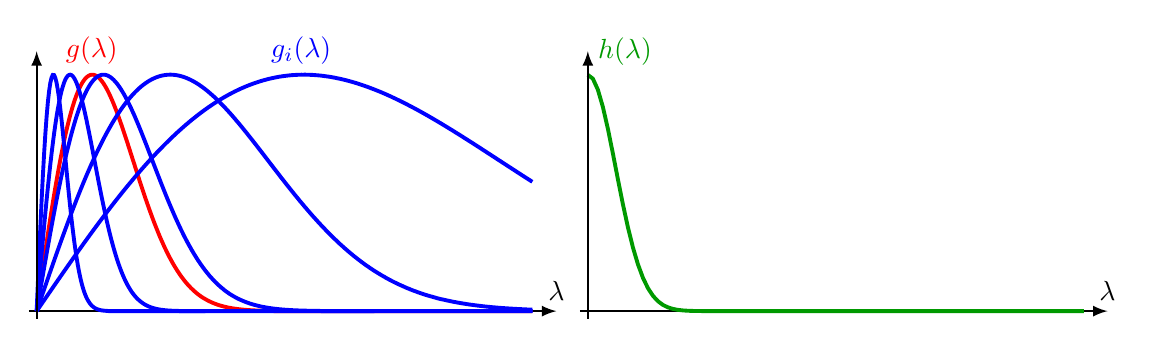
\begin{tikzpicture}[>=latex,thick]
\begin{scope}

\draw[->] (-0.1,0) -- (6.6,0) coordinate[label={$\lambda$}];

\kurve{1}{red}
\uncover<4->{
\foreach \k in {0,...,4}{
        \pgfmathparse{0.30*exp(ln(2)*\k)}
        \xdef\l{\pgfmathresult}
        \kurve{\l}{blue}
}
}

\node[color=red] at ({0.7*1},3) [above] {$g(\lambda)$};
\uncover<4->{
\node[color=blue] at ({0.7*0.3*16},3) [above] {$g_i(\lambda)$};
}

\draw[->] (0,-0.1) -- (0,3.3);
\end{scope}

\begin{scope}[xshift=7cm]

\uncover<6->{
\draw[->] (-0.1,0) -- (6.6,0) coordinate[label={$\lambda$}];

\draw[color=darkgreen,line width=1.4pt]
        plot[domain=0:6.3,samples=100]
                ({\x},{3*exp(-(\x/0.5)*(\x/0.5)});

\draw[->] (0,-0.1) -- (0,3.3) coordinate[label={right:$\color{darkgreen}h(\lambda)$}];
}

\end{scope}

\end{tikzpicture}
\end{center}
\end{frame}
\egroup
